\documentclass{article}
\usepackage[utf8]{inputenc}
\usepackage{graphicx}
\usepackage{xcolor}
\usepackage{pagecolor}
\usepackage{helvet}

\renewcommand{\familydefault}{\sfdefault}
% \pagecolor{black}
% \color{white}

\title{The City and The City}
\author{2023 Course Agenda}
\date{}

\begin{document}

\maketitle

\section{Course Agenda}


The workshop will emphasize world building through themes of automation and decentralization, constructing potential realities which include buildings and landscapes, as well as finer grain details that reveal behaviors and overall atmospheres through the use of video game engines. Each group will be assigned a specific city and examine its past, present, and future. Starting from a research-driven approach, a specific topic distinct to each city will be established and form the basis for determining what role architecture will play. Each team will design two things: 1) an architecture that responds to the local specifics of the city, 2) an interactive environment for their architecture to exist in. These two will be generated through a combination of simulations and generative algorithms that combine the excesses of data and materials in tandem will seek to manipulate current trends towards an alternate ending from what is currently predicted.

\section{Methodology / Research Direction}
Interactive Worlds (methodology/research agenda)
\newline \newline
When thinking of a particular place, we are indirectly thinking of a network of logistical, economical, cultural, environmental, and political processes. The course will be focused on using 'world building' and multi-dimensional narratives as a way to reveal the imminent possibilities of our near and/or distant futures. Using video game engines that combine simulations and interactivity, the workshop will revolve around the idea that "everything is connected" -- environment, people, material, and non-humans.

Some questions the workshop will investigate are:
\begin{itemize}
    \item How will infrastructure necessarily be created and/or adapted?
    \item What effects will this have on architectural production, habitation, and its environment?
    \item What role(s) will ubiquitous data and sentience play?
    \item What models of mitigation, resistance, and acceptance will result, and from who/what?
    \item How will these experiences be felt and through what mediums?
\end{itemize}

\section{Software / Skills Required}
A combination of:
\begin{itemize}
    \item Unreal - for interactive environments and video
    \item Rhino - for basic modeling
    \item Houdini and Blender - advanced modeling
    \item Adobe Premiere - short videos.
\end{itemize}

\section{Workflow Introduction}
\subsection{Research}
Each team will start with a detective wall that develops a series of relationships around particular \#hashtags – these will serve as entry points into a particular site or topic and will become the basis for speculation.

\subsection{Hashtags}
\#Decentralization, \#Automation, \#Artificiality, \#Artificial Intelligence, \#Copyright, \#Cloud Seeding/homogenitus, \#Archiving, \#Deforestation / Reforestation, \#Anthropocene / anthropogenic territories, \#Ferality, \#Carbon Offsetting, \#Decolonization, \#Non-Human, \#urk/urkopplad, \#plantation forests, \#antenna trees, \#Uncanny valley.
\newline \newline

Research on these keywords can be conducted between news articles, research papers, videos, etc. The idea is to move past the obvious information and devise connections and potential narratives.

\subsection{World Building the Real}
Teams will begin directly with building their worlds in the form of landscapes, architecture, and assets.

\subsection{Mutations / Speculations / Iterations}
Using the research, narratives will start to be developed that will guide the evolution of particular aspects of the world.

\subsection{Interactivity and Effects}
Interactive virtual environments will be created to test the performance of the devices/assets/architecture.

\subsection{Film Trailer Making}
Scene development and narrative building into a short movie combining multiple techniques (animations, compositing, etc.) to recount a future story from either one or multiple perspectives.

\section{Skills Schedule}
Skills are conducted by Jose Pareja-Gomez.

\subsection{Cinematics}
Date: July 23, 4 hrs

\subsection{Interactions}
Date: July 30, 4 hrs

\subsection{AR and Specifics}
August 6, 4 hrs

\section{General Schedule}
Hadin - Tuesdays at 8:00-11:00 China time (17:00-20:00)

Joris - Fridays at [insert time]

\begin{itemize}
    \item July 15 - first class
    \item August 6 - midterm (around then)
    \item September 11 - final
\end{itemize}

\section{Reading List}
\begin{itemize}
    \item Machine Landscapes, Liam Young
    \item The Estranged Object, edited by Young + Ayata
    \item Planet City, Liam Young
    \item Dark Ecology, Timothy Morton
    \item ...
\end{itemize}

\section{Watching List}
\begin{itemize}
    \item \url{https://www.youtube.com/watch?v=rE_c0hmx9Fg}
    \item Sdsd
    \item Add whatever you think
\end{itemize}

\section{Reference Projects (from BPro)}
\begin{itemize}
    \item ACRE
    \item LIVES
    \item Gaming Consensus
    \item Arctic Everywhere
\end{itemize}

\section{General Schedule for Student Development}
Note: Skills may shift around depending on progress.

\textbf{Week 1 (07/15)} - INTRO TO PAST YEAR + DETECTIVE WALL + SKILLS

Overview of how last year's projects evolved.
Research into assigned city/topic and climate/socio-political projection.
Initial skill development of collaborative functionalities by making a small world in Unreal. Bringing in assets, making an asset, and controlling lighting.
First assignment – recreate a scene and specific shot from an assigned video.
\newline
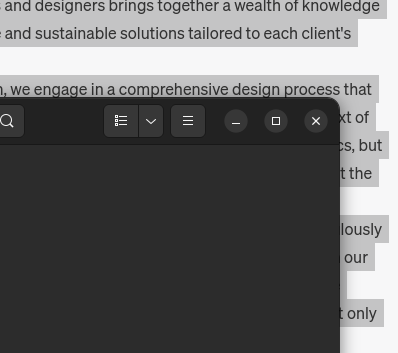
\includegraphics[width=1\textwidth]{a.png}

\end{document}
